\documentclass{article}
\usepackage{graphicx}
\usepackage{hyperref}
\usepackage{fancyvrb}
\usepackage{vhistory}
\usepackage{float}
\hypersetup{colorlinks,urlcolor=red}
\usepackage[margin=1in]{geometry}
\usepackage{listing}
\usepackage{url}

\usepackage{amsmath}
\usepackage{amssymb}
\usepackage{amsthm}
\usepackage{mathtools} %for use of := symbol mostly.
\usepackage{booktabs} % used for making tables

\usepackage[export]{adjustbox} % allows frame around figure

\usepackage[round]{natbib}


\newcommand{\pnote}[1]{{\langle \text{#1} \rangle}}

\begin{document}

\title{\textbf{TrawlExpert: Tool for Watershed Biological Research}}
\author{Trawlstars Inc. (Group 11) \\ Lab section: L01  \\ Version: 1.0 \\ SFWRENG 2XB3 \\ \\ Christopher W. Schankula, 400026650, schankuc \\ Haley Glavina, 001412343, glavinhc \\ Winnie Liang, 400074498, liangw15 \\ Ray Liu, 400055250, liuc40 \\ Lawrence Chung, 400014482, chungl1}

\maketitle

\newpage

\begin{versionhistory}
  \vhEntry{1.0}{05.04.18}{HG}{created}
  \vhEntry{1.1}{08.04.18}{HG}{algorithmic analysis added}
\end{versionhistory} 

\noindent\textit{By virtue of submitting this document we electronically sign and date that the work being submitted by all the individuals in the group is their exclusive work as a group and we consent to make available the application being developed through SE-2XB3 project, the reports, presentations, and assignments (not including my name and student number) for future teaching purposes.}

\newpage

\textbf{\Large{Team Contributions}}\\ \\
The individual contributions of each team member are described below. Subteam B indicates an algorithmic focus in a member's efforts while Subteam A indicates a focus on data parsing and user interface development. Although the contributions have been separated such that each task is recorded under one contributor, members often overlapped duties and designed modules together. \\

\begin{table}[h]
	\centering
	\begin{tabular}{p{0.16\hsize}p{0.38\hsize}p{0.38\hsize}}
		\toprule
		\textbf{Name} & \textbf{Role} & \textbf{Contributions}\\
		\midrule
		Lawrence Chung\\
		& Head of Room Booking \newline Subteam B Member
		& Implemented the depth first search and connected components algorithms. \\
		\midrule
		Haley Glavina\\
		& Meeting Minutes Administrator \newline Subteam B Member
		& Implemented the red-black tree, quickselect, and mergesort algorithms. Designed the final presentation powerpoint, recorded and submitted all meeting minutes, and assembled the final design specification in LaTeX.\\
		\midrule
		Winnie Liang\\
		& Project Log Administrator \newline Subteam A Member
		& Implemented the module responsible for parsing out data to create related objects, implemented taxonNode ADT. Led user interface development, set up tomcat files and directory structure,  handled communication between the Google Maps APIs and javascript code. Overlooked project log entries.\\
		\midrule
		Ray Liu\\
		& TA \& Professor Liaison \newline Subteam A Member
		& Implemented Record ADT, Date ADT, parsing API calls for WORM API, RangeHelper for Basic Search, Histogram.\\
		\midrule
		Christopher Schankula\\
		& Team Leader \newline Subteam A Member
		& Determined the goals for each meeting, implemented the k-d tree algorithm, and handled server communication. \\		
		\bottomrule
	\end{tabular}
\end{table}


\newpage

\begin{abstract}
\noindent \textit{TrawlExpert} is a powerful tool to enable researchers to analyze and filter large datasets from fish trawl surveys in order to perform environmental research on fish and invertebrate populations. The tool gives researchers the ability to intelligently filter and query datasets based on biological classification such as family, genus or species, or based on location or timeframe. Advanced outputs display data as a histogram or geographical map, each depending on population abundance as a function of time and spatial distribution. Additionally, \textit{TrawlExpert} provides a tool for finding local subpopulations within a larger query. A dataset of thousands of Great Lakes trawl surveys from 1958-2016 will be used as a demonstration of \textit{TrawlExpert}'s capability to help researchers narrow down large datasets and glean data which pertains to their research. \textit{TrawlExpert} will be designed to be used easily and effectively as the first step in a groundbreaking climate and ecological research pipeline.
\end{abstract}


\tableofcontents


\section{Project Scope}
\subsection{Objective}
Provide a statistical and visual tool for the analysis of water ecosystems, based on scientific water trawl data. Gives researchers with tools to analyze large datasets to find patterns in fish populations, including the plotting of historical population data on a map, the analysis of population trends over time and the determination of subpopulations of a certain biological classification.

\subsection{Motivation}
The diminishing of fish populations in the Great Lakes became a problem in the latter half of the 20th century, with the total prey fish biomass declining in Lakes Superior, Michigan, Huron and Ontario between 1978 and 2015 \citep{michigan2017}. Annual bottom trawl surveys involve using specialized equipment to sweep an area and are used to determine the relative temporal variation in stock size, mortality and birth rates of different fish species \citep{walsh1997efficiency}. These surveys are performed annually and often have hundreds of thousands of records, making manual analysis infeasible. The ongoing protection and development of the Great Lakes water basins is considered an important topic for scientists in both Canada and the United States, as evidenced by grants such as the \textit{Michigan Sea Grant} \citep{michseagr2018}.

TrawlExpert will give researchers tools to filter through these large amounts of data by allowing them to search through data based on class, order, genus, family or species. This will help support scientific researchers and fishing companies as they study fish populations. These studies help inform initiatives to preserve fish populations and conduct their business in an environmentally friendly way going forward. As more data is collected on an annual basis, TrawlExpert can easily be injected with the new data and will adjust and scale accordingly, combining the new data with the old data for continued analysis.

TrawlExpert will also analyze the trawl data to find connected subpopulations within the data, giving researchers tools to analyze the portions of the water body that contain different populations and even track these specific subpopulations over time.

The focus of the project will be to develop these unique data searching and querying tools as a first step in a complete trawl survey analysis. For a complete analysis, tools like stratified statistical analysis are required by the researcher \citep{walsh1997efficiency}. For purposes of maintaining a manageable scope for this project, the implementation of advanced trawl survey scientific and statistical analysis tools will be relegated to future developments. 

\subsection{Dataset}\label{sec:out}
The test dataset that will be used for purposes of this project is the \textit{USGS Great Lakes Science Center Research Vessel Catch Information System Trawl} published by the United States Geological Survey \citep{usgs2018}. Compiled on yearly operations taking place from early spring to late fall from 1958 until 2016, the dataset contains over 283,000 trawl survey records in the five Great Lakes, including the latitude and longitude co-ordinates and biological classification such as family, genus and species.

\section{Implementation}
\subsection{Classes and Modules}
The implementation involved over 30 classes implemented in Java. Additional JavaScript and html files were used to create a sophisticated user interface. For a description of each class and module used, Java documentation can be viewed at %INSERT JAVA DOC LINK% 

\subsection{Class Organization}
The following UML diagrams depict the organization and use-relations of all classes in the program. Two UML state machine diagrams are included to describe the states and transitions within the \textit{BioTree.java} and \textit{Main.java} class. Since the \textit{Main.java} class is a console version of the final server implementation, the states shown in its UML state machine diagram are analogous to the states of the final \textit{TrawlExpert} product.

% Include explanations of why we divided it into some of its main sections/classes

\begin{figure}[H]
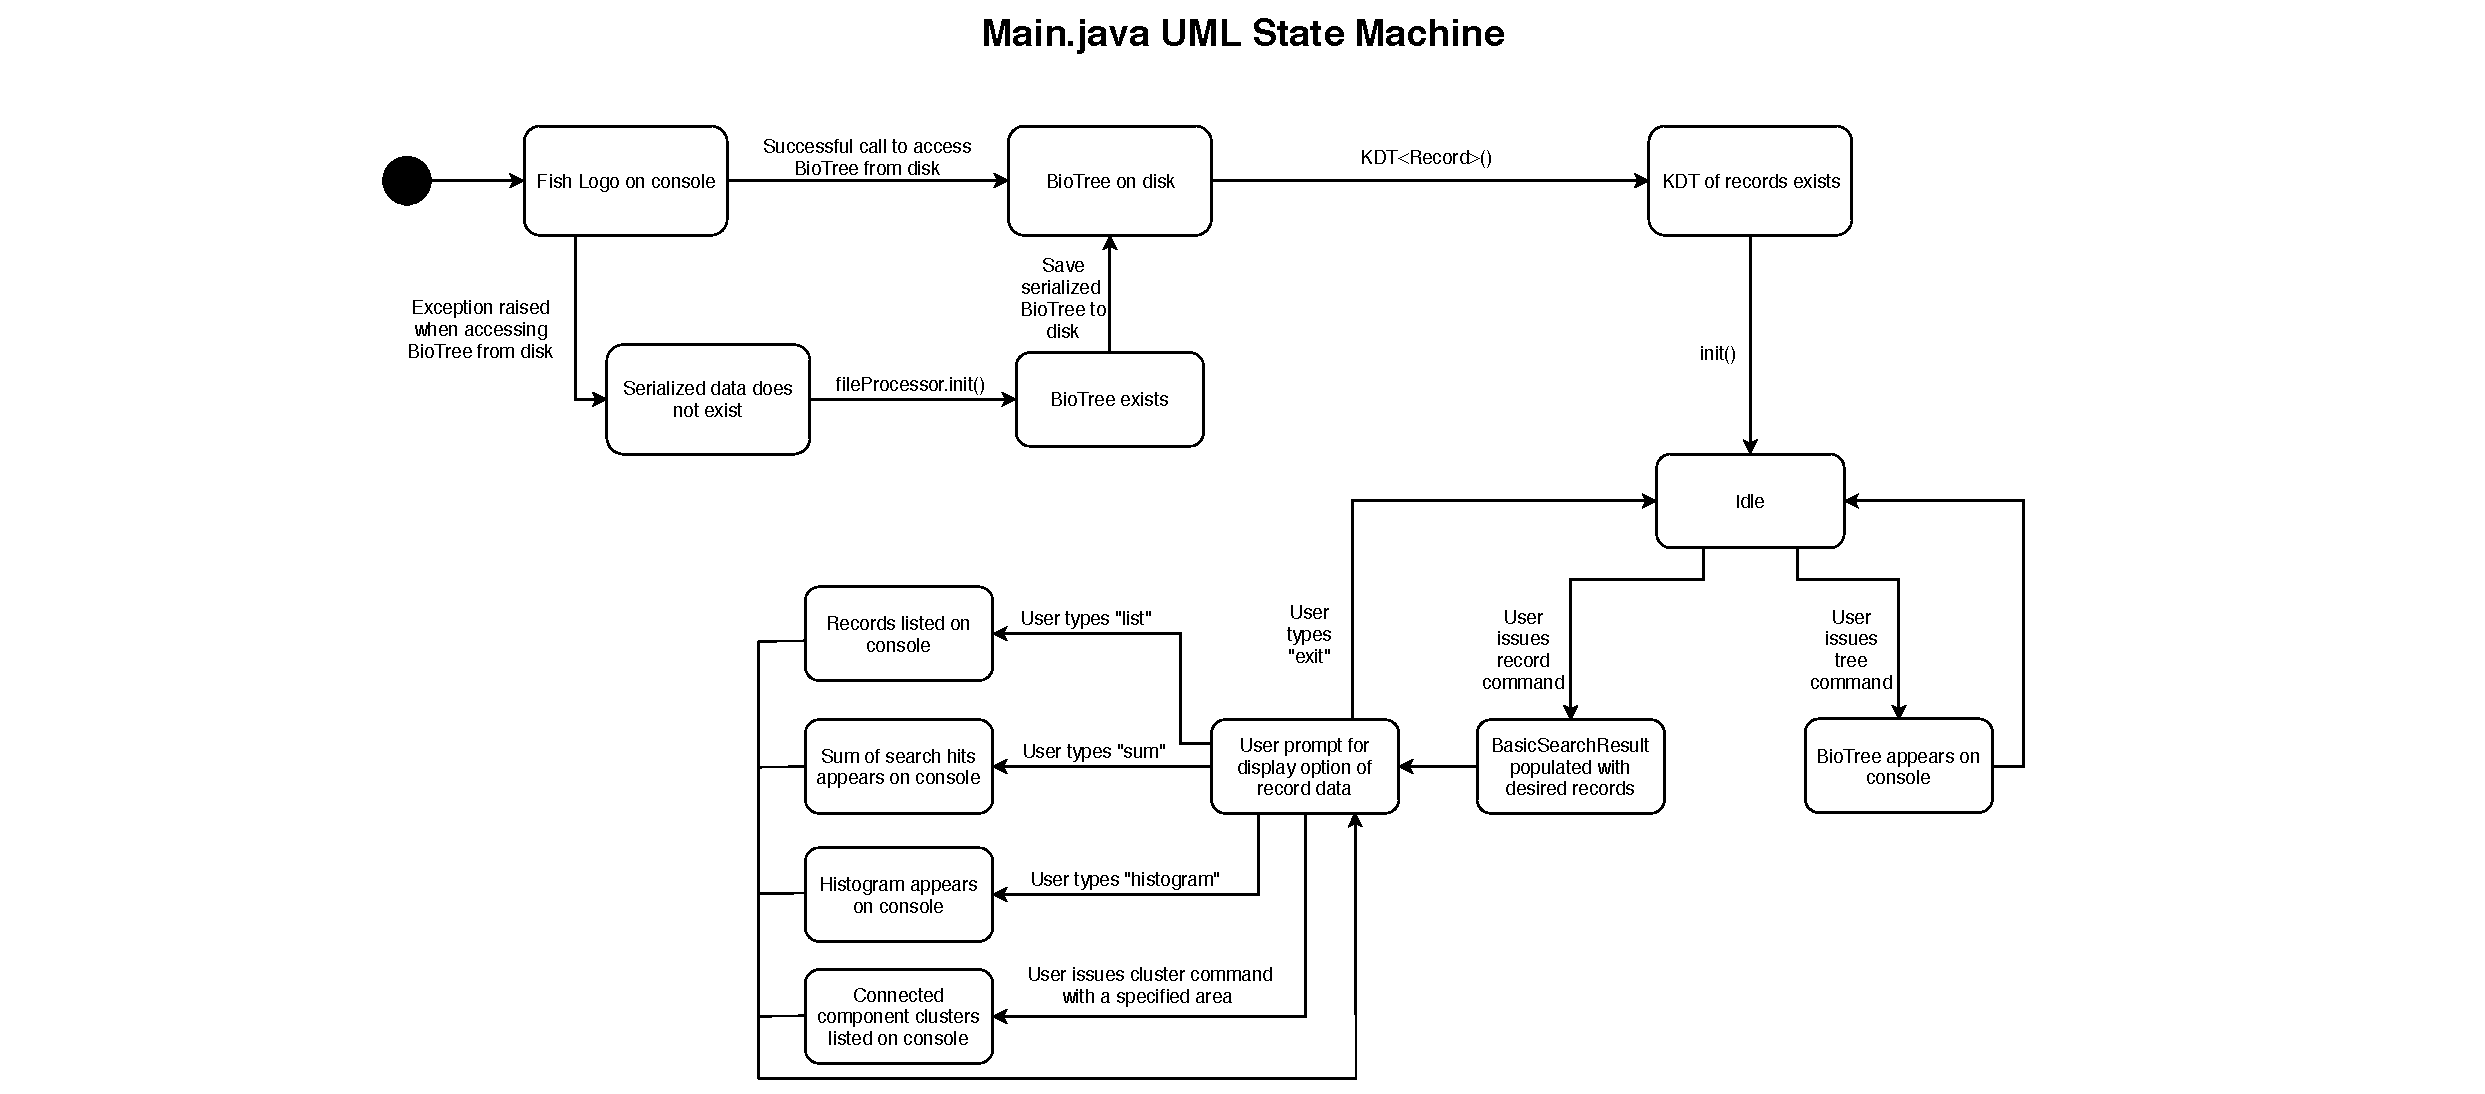
\includegraphics[width=18cm, trim={6cm 0 6cm 0}, clip]{MainDotJava.pdf}
\caption{UML State machine diagram for \textit{Main.java}, a class that provides console access to the \textit{TrawlExpert}'s main functions. This class accepts search criteria from a user to produce a list of search results, depict a histogram of the records in that result, and compute a count of the search hits.}
\label{fig:Tree}
\end{figure}

\subsection{Maintaining Generality}
\subsubsection{General Compare}
A common theme among \textit{TrawlExpert} classes is the use of lambda functions. Lambda functions provide the capacity for parameterized object comparison or parameterized value access. This maintains the generality, and therefore reusability, of each class. 

The \textit{GeneralCompare} interface can be found at \textit{/sort/GeneralCompare.java}. The interface includes a compare function that takes two generally typed inputs and produces an integer output. When \textit{GeneralCompare} is used in other classes, a compare function (the lambda function) is used to instantiate the expected input type and designate how the integer result must be calculated. This allows reuse of the interface among modules that perform comparisons of differently typed objects. Two records consisting of a fish species, date of observation, and geographic location can be compared based on lexicographic order of their names, date, or proximity to some location. \textit{GeneralCompare} enables the comparison of record objects based on any of these parameters. 

\subsubsection{Field}

\subsubsection{General Range}
% Similar to gc but 
% The range itself is the lambda function
% Input is a single object
% Returns int describing if obj is in that range (-1 = below lower bound, 0 = in bounds, or 1 = above upper bound)

\section{Algorithmic Opportunities}
\subsection{Quick Select Algorithm}
A modified form of binary search will be used for quickly locating the first of a given key in the large dataset and will be a crucial building block of all three main types of output. This will allow all entries of a given query to be found.

\subsection{K-d Tree Algorithm}
% Chris will write :) 

\subsection{Graph Algorithms}
Graph algorithms were used to support advanced searching features. Firstly, the biological classification of each organism forms a tree from which species in the same genus, for example, can be located. 

Secondly, a graph algorithm was used to find connected components among search results. Nodes are connected together based on their distance to surrounding points \citep{tom10}. Depth-first search was used to determine connected components \citep{broder2000graph}.

\clearpage
\section{Project Plan}
\subsection{Milestones}
The following milestones will help inform our progress towards completing the goals. Given that the team contains 5 people, the team will be divided up into two subteams of 2-3 people for maximum efficiency. Individual members' tasks can be decided by the subteams based on the progress of that team towards completing the next milestone's goal(s). Subteams should be in constant communication and in agreement about the inputs and outputs of modules to avoid the need rewriting of code.


\begin{table}[h]
	\centering
	\begin{tabular}{p{0.16\hsize}p{0.38\hsize}p{0.38\hsize}}
		\toprule
		\textbf{Milestone} & \textbf{Subteam A} & \textbf{Subteam B}\\
		\midrule
		Milestone 1 \newline (``Bedrock'') \newline(End of Week 1)
		& Finished parsing module for .csv data to create Java objects that can be used for analysis; start data cleansing
		& General binary search module underway \\
		\midrule
		Milestone 2 \newline (``Quartz'') \newline(End of Week 2)
		& Cleansed the data to remove or correct entries not containing all of the columns; start generating biological classification tree module
		& Finished and tested binary search; start mergesort \\
		\midrule
		Milestone 3 \newline (``Granite'') \newline(End of Week 4)
		& Finished and tested biological classification tree; start formatted text output
		& Finished and tested mergesort; start writing query module for output type 1, 2 and 3 making use of the biological classification tree, mergesort and binary search to get results from data \\
		\midrule
		Milestone 4 \newline (``Sandstone'') \newline(End of Week 6)
		& Continue text output tools. Google Maps API should be explored if time allows, otherwise it can be omitted to keep the project within scope
		& Continue query module: finished output 1,  2 \& 2; start output type 4\\
		\midrule
		Milestone 5 \newline (``Diamond'') \newline(End of Week 8)
		& Finished data visualization or text output tools; prepare keynote presentation
		& Finished output type 4; prepare keynote presentation \\		
		\bottomrule
	\end{tabular}
\end{table}

\noindent While this schedule provides a good reference and a way to monitor progress, team members should be flexible and remain in communication to ensure the project is kept on schedule. For example, if a milestone is reached before its given date, the next milestone should start development early. Approximately 1-2 weeks have been purposely left as padding at the end in case of unforeseen circumstances.


\subsection{Team Roles}
\begin{table}[h]
	\centering
	\begin{tabular}{p{0.20\hsize}p{0.30\hsize}p{0.10\hsize}}
		\toprule
		\textbf{Member} & \textbf{Role} & \textbf{Subteam}\\
		\midrule
		Christoper Schankula & Team Lead & A\\		
		\midrule
		Ray Liu & TA \& Professor Liaison & A\\	
		\midrule
		Winning Liang & Project Log Admin & A\\		
		\midrule
		Haley Glavina & Meeting Minutes Admin & B\\	
		\midrule
		Lawrence Chung & Head of Booking & B\\
		\bottomrule
	\end{tabular}
\end{table}

\subsection{Workflow}

The team will use \textbf{GitLab} as the primary way of sharing code and keeping up to date. The Git repository will be split into two branches, in addition to the \textit{master} branch: \textit{TeamA} and \textit{TeamB}. Each Subteam will develop on their respective branch, then issue merge requests so the team can evaluate and approve merges into the \textit{master} branch.

\subsection{Communication}

The team will use \textbf{Slack} and \textbf{Facebook Messenger} as primary and secondary means of communication. A Slack group has been created and each of the members were invited to it. \textbf{Google Drive} will be used to keep track of documentation such as the \textit{Project Log} and meeting minutes.

\clearpage
\bibliographystyle{apa}
\bibliography{bib}


\end{document}